\documentclass{article}

% URLs and hyperlinks ---------------------------------------
\usepackage{hyperref}
\hypersetup{
    colorlinks=true,
    linkcolor=blue,
    filecolor=magenta,      
    urlcolor=black,
}
\usepackage{xurl}
%----------------------------------------------------

\usepackage{graphicx}
\usepackage{float}

\usepackage{xepersian}
\settextfont{Yas}

\title{تکلیف اول}
\author{مهدی حق‌وردی}
\date{\today}

\begin{document}
\maketitle
\tableofcontents

\section{سوال اول - شکستن متن شنود شده}
متن شنود شده را توسط کدی که در اینجا\LTRfootnote{\url{https://github.com/mahdihaghverdi/cryptography/tree/main/affine_break}}
وجود دارد را با تمامی کلید‌‌های ممکن امتحان کردم و هر کدام از خروجی‌ها را بررسی کردم که به این رسیدم:
\begin{figure}[H]
\begin{center}
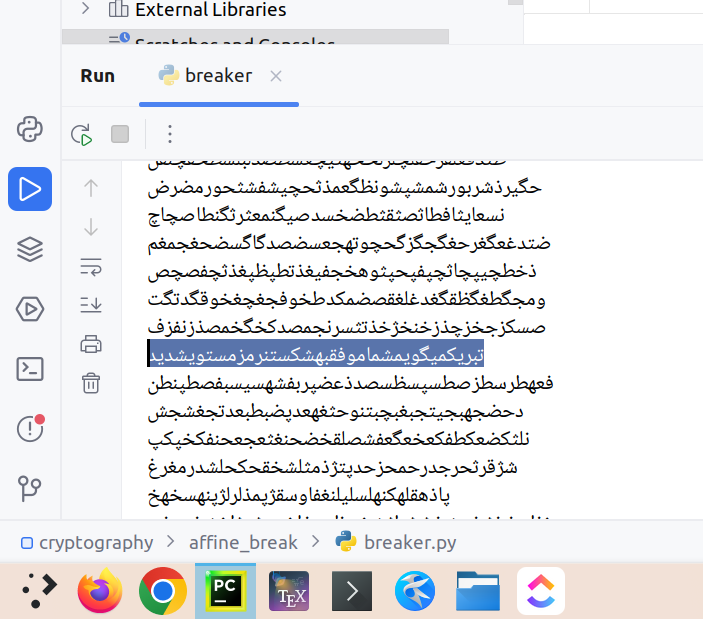
\includegraphics[width=0.6\textwidth, height=0.4\textheight]{images/found}
\end{center}
\end{figure}

\subsection{توضیحات کد}

\begin{itemize}
\item 
\lr{\texttt{pre\_needed.py}}

مقادیری که این ماژول وجود دارند مقادیری مانند الفبای فارسی، تمام کلید‌ها و یک سری ثابت هستند که در برنامه برای رمزنگاری و رمزگشایی به آنها نیاز است.

\item \lr{\texttt{functions.py}}

توابعی که در این ماژول هستند دو تابع 
\lr{\texttt{encode}}
و
\lr{\texttt{decode}}
هستند که طبق فرمول‌های رمز مستوی نوشته شده‌اند.

\item \lr{\texttt{breaker.py}}

در این ماژول در حلقه‌ی 
\lr{\texttt{for}}
اول، متن رمزشده را با تمامی کلید‌های ممکن رمزگشایی کرده و نتیجه را پرینت می‌کنیم و سپس در خروجی به دنبال یک متن معنی دار می‌گردیم.

حالا برای پیدا کردن کلید هم می‌توانیم بین کلید‌ها بگردیم و آن کلیدی که متن با آن رمز شده را پیدا کنیم که آن کلید:
\lr{\texttt{Key(a=5, b=3)}}
است.
\end{itemize}
\end{document}